\documentclass[usenatbib,onecolumn,galley]{mn2e}
\usepackage{graphicx}
\usepackage{amsmath}
\usepackage{mathrsfs}

\newcommand{\Glass}{{\sc Glass}}
\newcommand{\PixeLens}{{\sc PixeLens}}
\newcommand{\Rmap}{\ensuremath{R_\mathrm{map}}}
\newcommand{\Rpix}{\ensuremath{R_\mathrm{pix}}}
\newcommand{\M}{\ensuremath{\mathscr{M}}}
\newcommand{\E}{\ensuremath{\mathscr{E}}}
\newcommand{\eps}{\ensuremath{\varepsilon}}
\newcommand{\Eavg}{\ensuremath{\langle \E \rangle}}
\newcommand{\kpc}{\ensuremath{\mathrm{kpc}}}
\newcommand{\Msun}{\ensuremath{\mathrm{M}_\odot}}
\newcommand{\tabref}[1] {Table~\ref{#1}}
\newcommand{\figref}[1] {Figure~\ref{#1}}
\newcommand{\eqnref}[1] {Eq.~(\ref{#1})}
\newcommand{\secref}[1] {Section~\ref{#1}}
\newcommand{\appref}[1] {Appendix~\ref{#1}}
\newcommand{\e}[1]{\ensuremath{\times 10^{#1}}}
\renewcommand{\vec}[1]{\ensuremath{\boldsymbol{#1}}}


\title{Gravitational-Lens Recovery with GLASS}
\author{%
Jonathan P. Coles 
\and 
Justin I. Read
\and 
Prasenjit Saha 
}

\begin{document}
\maketitle

\begin{abstract}
\end{abstract}

\section{Introduction}

\section{GLASS}

Extensible framework, with some new features: (i) sampling algorithm
from \cite{2012MNRAS.425.3077L}, (ii) stellar mass as lower limit,
(iii) central high-resolution region, (iv) post-processing using
kinematics.

\begin{equation}
\vec\beta = \vec\theta - \frac{D_{LS}}{D_S} \times \frac{4GD_L}{c^2}
\int \Sigma(\vec\theta')
\frac{(\vec\theta - \vec\theta')}{\ |\vec\theta - \vec\theta'|^2}
d^2\vec\theta'
\label{lensing equation}
\end{equation}

\begin{equation}
\frac{ct(\vec\theta)}{(1+z_L)D_{L}} =
\frac{D_{S}}{D_{LS}} \times {\textstyle\frac12} |\vec\theta - \vec\beta|^2
- \frac{4GD_{L}}{c^2}
\int \Sigma(\vec\theta') \ln |\vec\theta-\vec\theta'| d^2\vec\theta'
\label{full arrival time}
\end{equation}
\begin{equation}
D_L, D_S, D_{LS} \propto \frac c{H_0}
\end{equation}

\section{Simulated Lenses}

Triaxial models with stars and dark matter.
\begin{equation}
\rho(r) = \frac{M}{4\pi a^3}(3-\gamma)
\left(\frac ra\right)^{-\gamma}\left(1 + \frac ra\right)^{\gamma-4}
\label{Dehnen profile}
\end{equation}
Steep and shallow light, steep and shallow dark-matter: \tabref{mock
  galaxy params} and \figref{mock galaxies}.

\begin{table}
\begin{center}
\begin{tabular}{cllllllll}
Galaxy & $\gamma_\star$ & $M_\star$ & $\gamma_\mathrm{DM}$ & $M_\mathrm{DM}$ & $\Rmap$ & Notes\\
\hline
AA & 1 & 4 & 0.05 & $11^{2.95}$ & 50 kpc & \\
AC & 1 & 4 & 1 & $11^2$ & 50 kpc & \\
BB & 1.5 & $2^{1.5}$ & 0.16 & $11^{2.84}$ & 50 kpc & \\
BC & 1.5 & $2^{1.5}$ & 1 & $11^2$ & 10 kpc & 
\end{tabular}
\end{center}
\caption{Profile parameters for the four mock galaxies. The resulting profiles only roughly follow
\eqnref{Dehnen profile} because the galaxies are triaxial. Masses are in units of $1.8\e{10}\Msun$. The scale lengths for
all lenses are $(a_\star,a_\mathrm{DM})=(2,20)$ kpc and by definition
$M_\star(a_\star) = M_\mathrm{DM}(a_\star) = 1$. $\Rmap$ is the 2d projected radius used to generate the lens configurations.}
\label{mock galaxy params}
\end{table}

\begin{figure}
\begin{center}
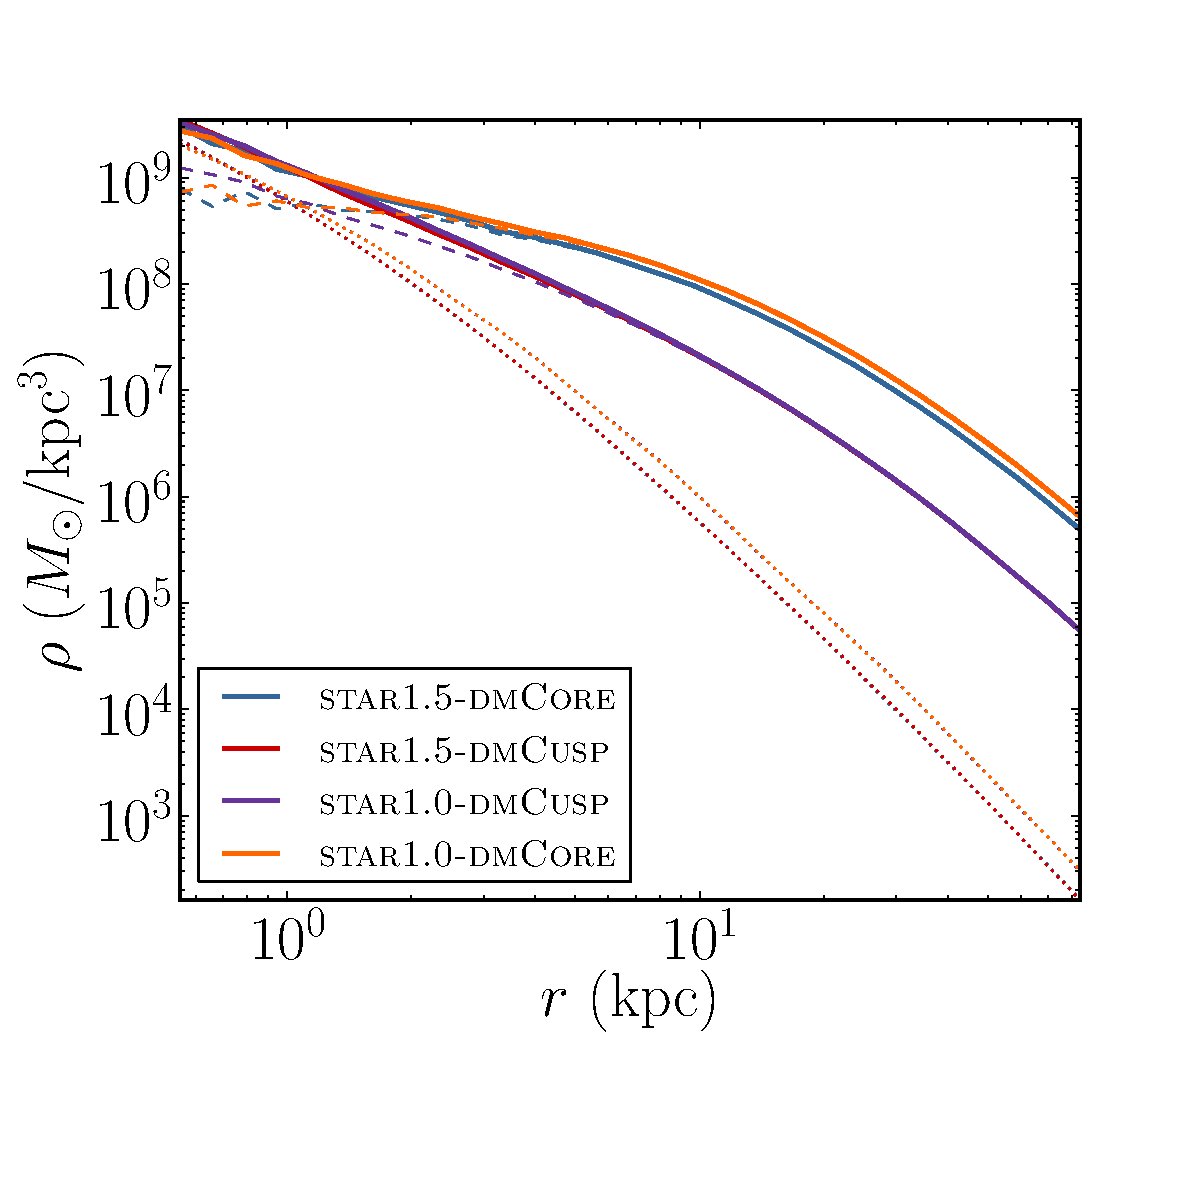
\includegraphics[width=.5\columnwidth]{MockGalProfile-a.pdf}
\end{center}
\caption{Three-dimensional density of the galaxies showing the
  stellar, dark matter, and total densities with dotted, dashed, and
  solid lines, respectively.}
\label{mock galaxies}
\end{figure}

Then project galaxies to get lenses, \figref{mock lenses}.

\begin{figure}
\begin{center}
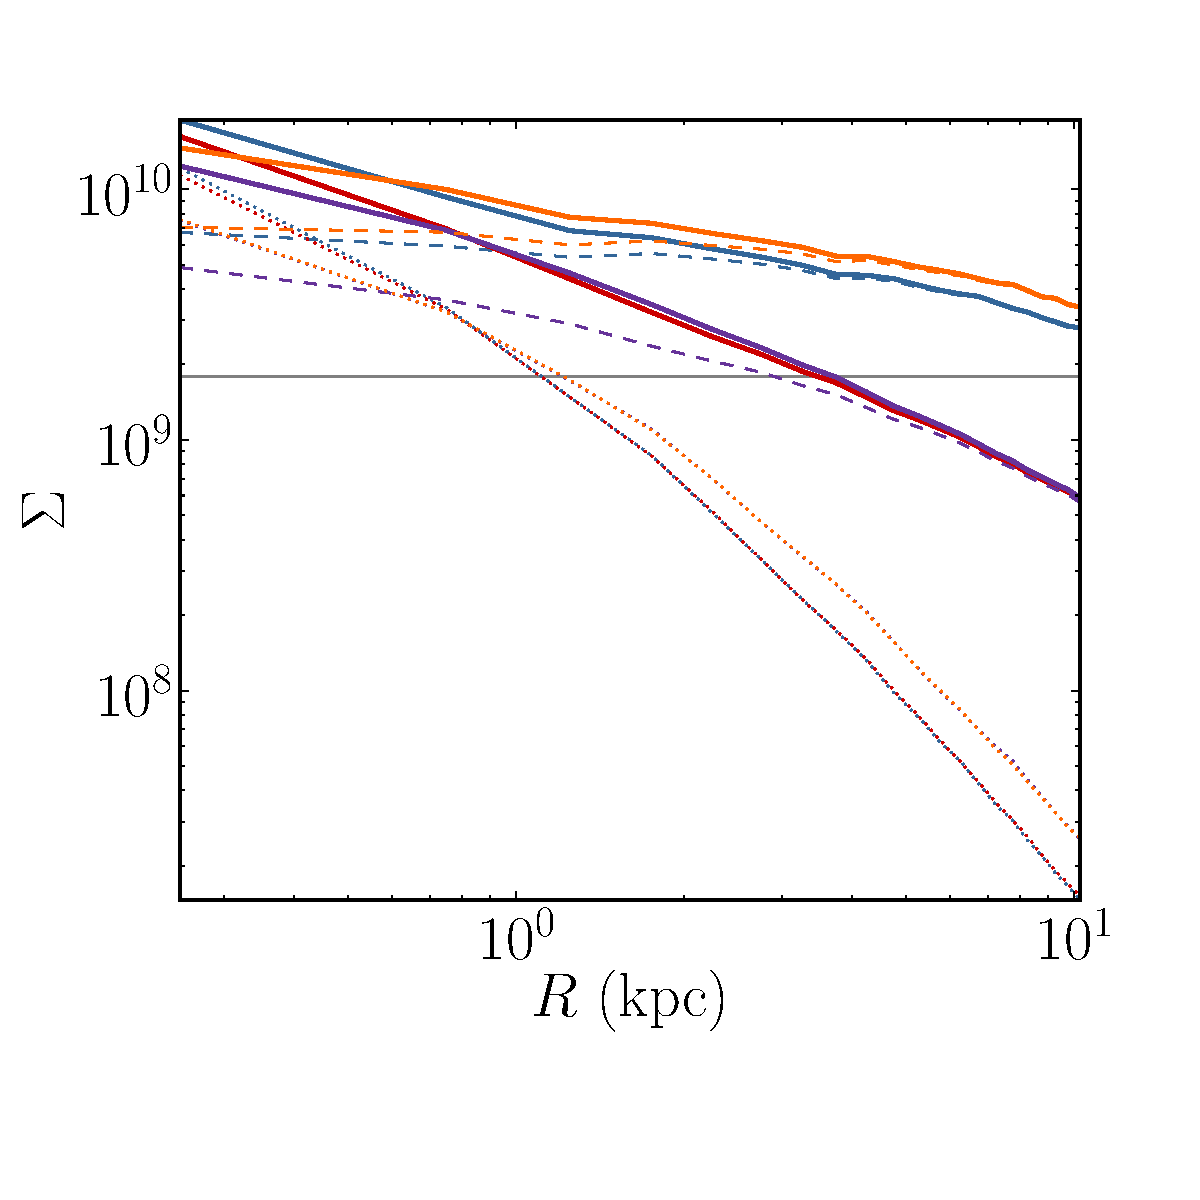
\includegraphics[width=.5\columnwidth]{MockGalProfile-b.pdf}\break
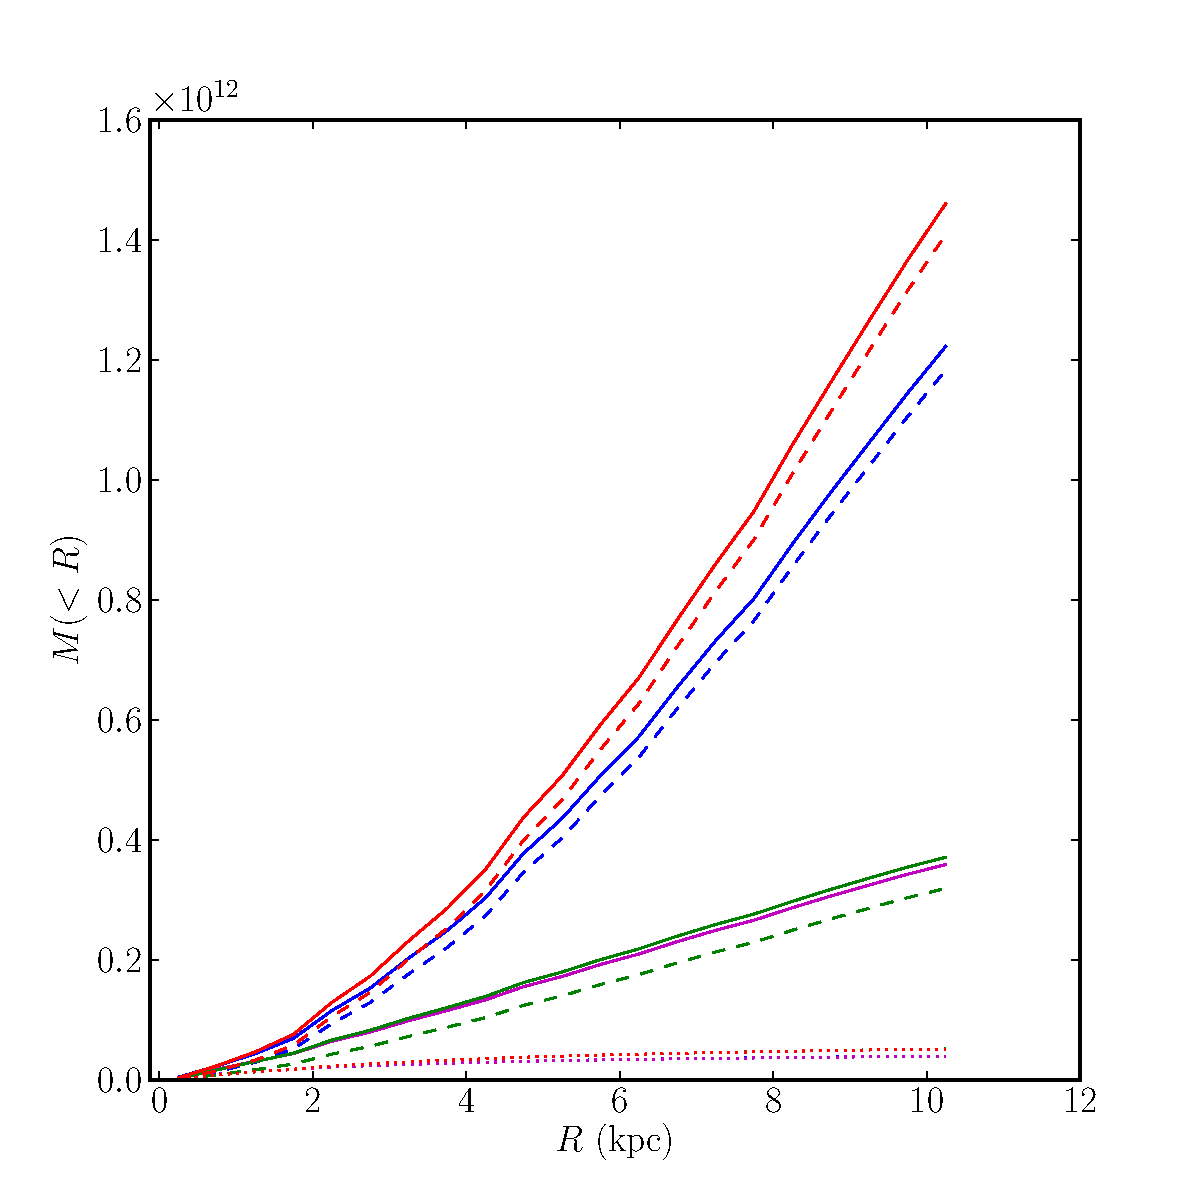
\includegraphics[width=.5\columnwidth]{MockGalProfile-c.pdf}
\end{center}
\caption{The radially averaged two-dimensional projected density and
  enclosed mass.  The critical density for lensing at $z_L=0.31$ is
  $\Sigma_\mathrm{crit}\sim 1.8\e{9}$\Msun/kpc$^2$.}
\label{mock lenses}
\end{figure}

\begin{figure}
\begin{center}
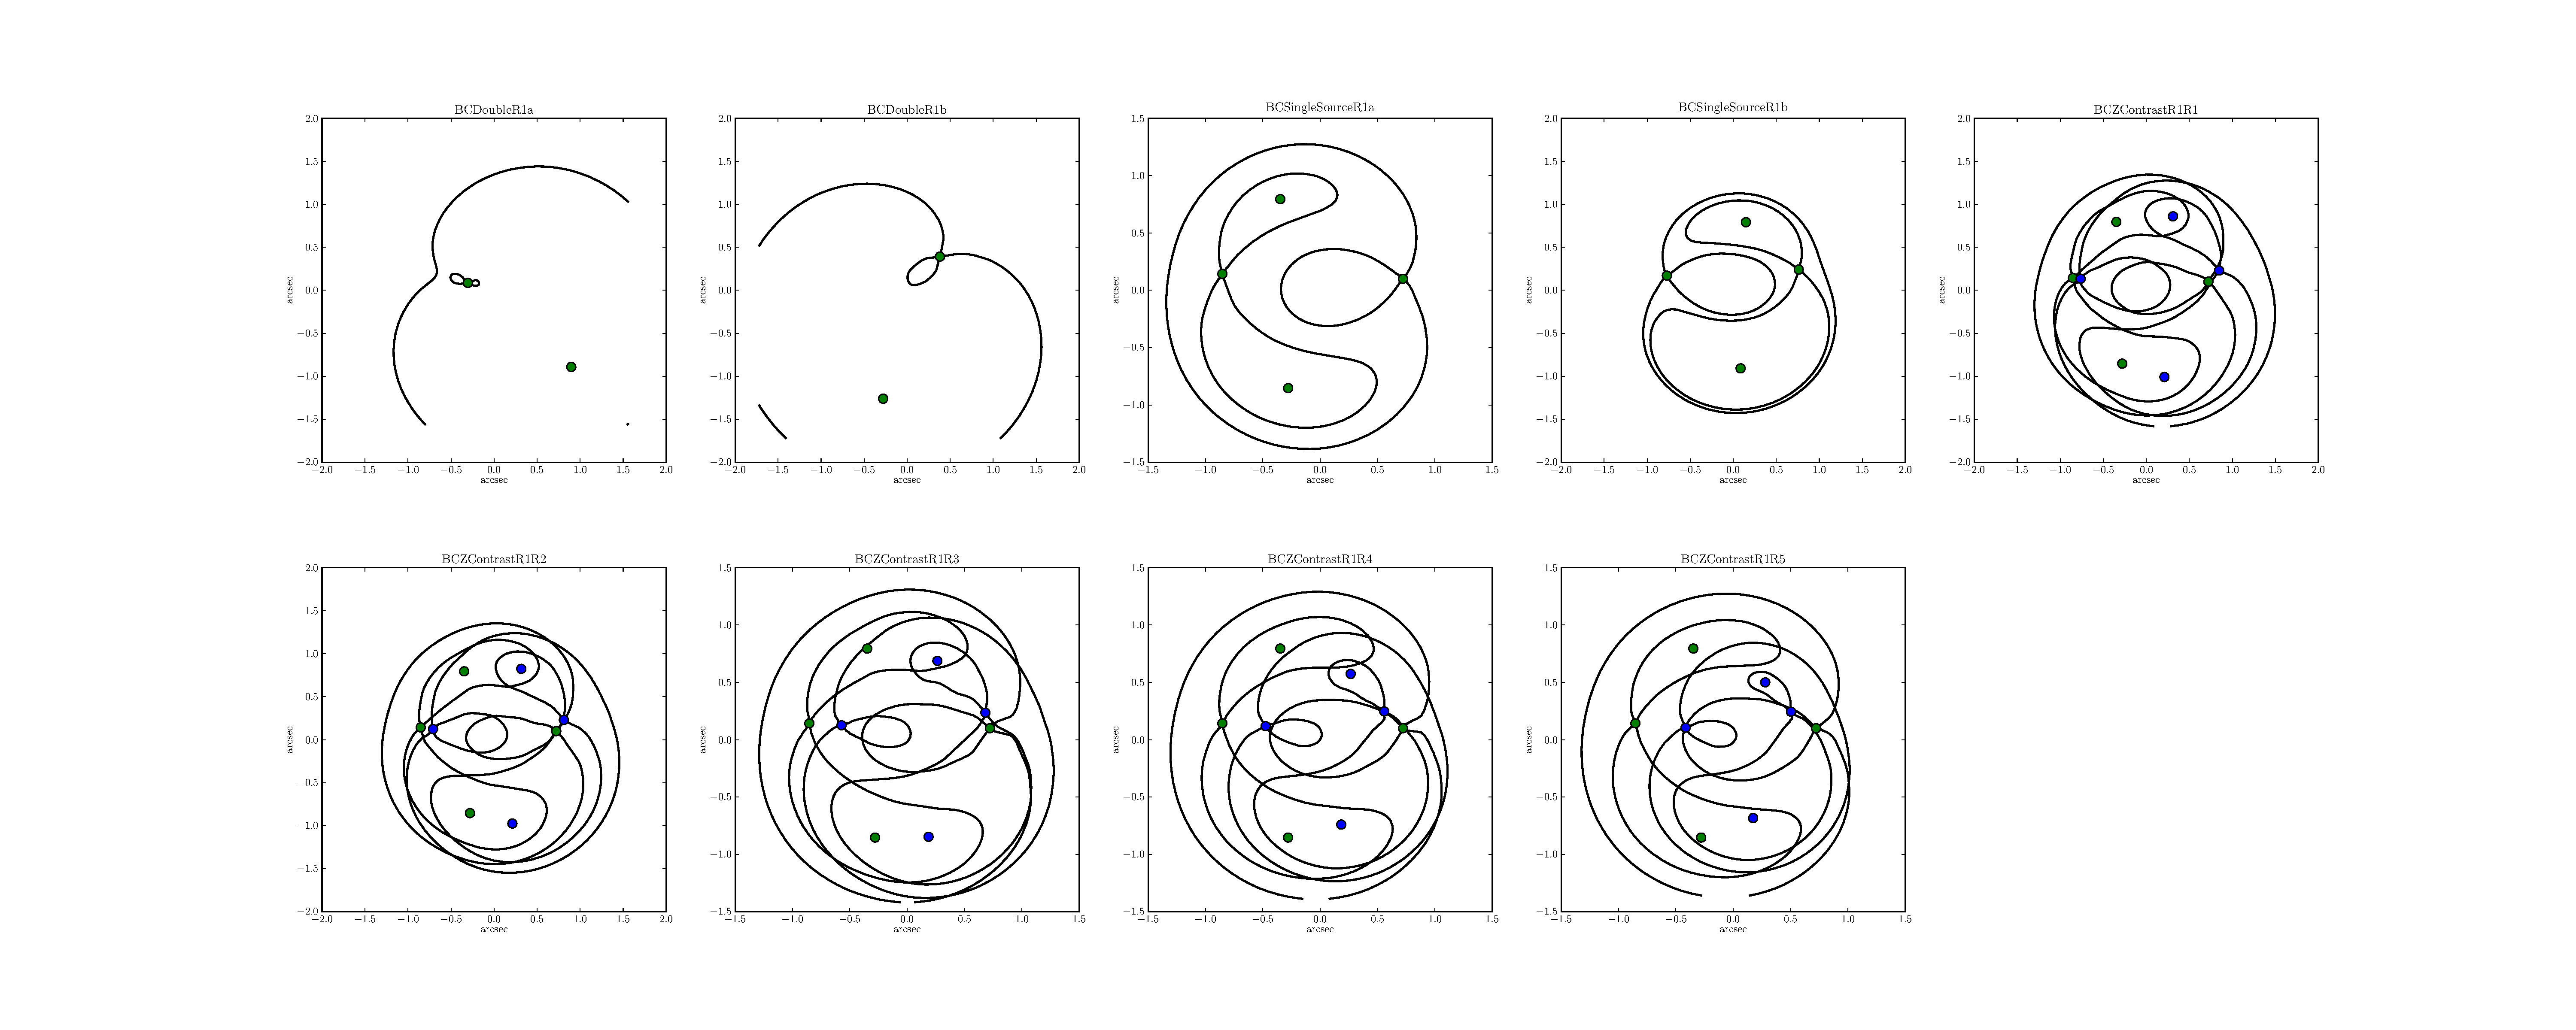
\includegraphics[width=.8\columnwidth]{BCarrival_surfaces}
\end{center}
\caption{The lens configurations for the six test cases using the BC
  mock galaxy.}
%  Here, the central image is shown, although not all
% tests include it. The central image belongs to only one set of
% images to avoid overconstraining the models. Similar colors group
% imagethat share a common source. In the case of the extended image
% systems the source is at the same redshift, while the redshift is
% varied between the systems in the ZConstrast cases. Grey circles are
% a visual aid to help determine radial separation between images. The
% axes are measure in arcseconds.}
\label{reconstruction}
\end{figure}

Convergence test for ray-tracing, \figref{raytracing convergence
  tests}.

\begin{figure}
\begin{center}
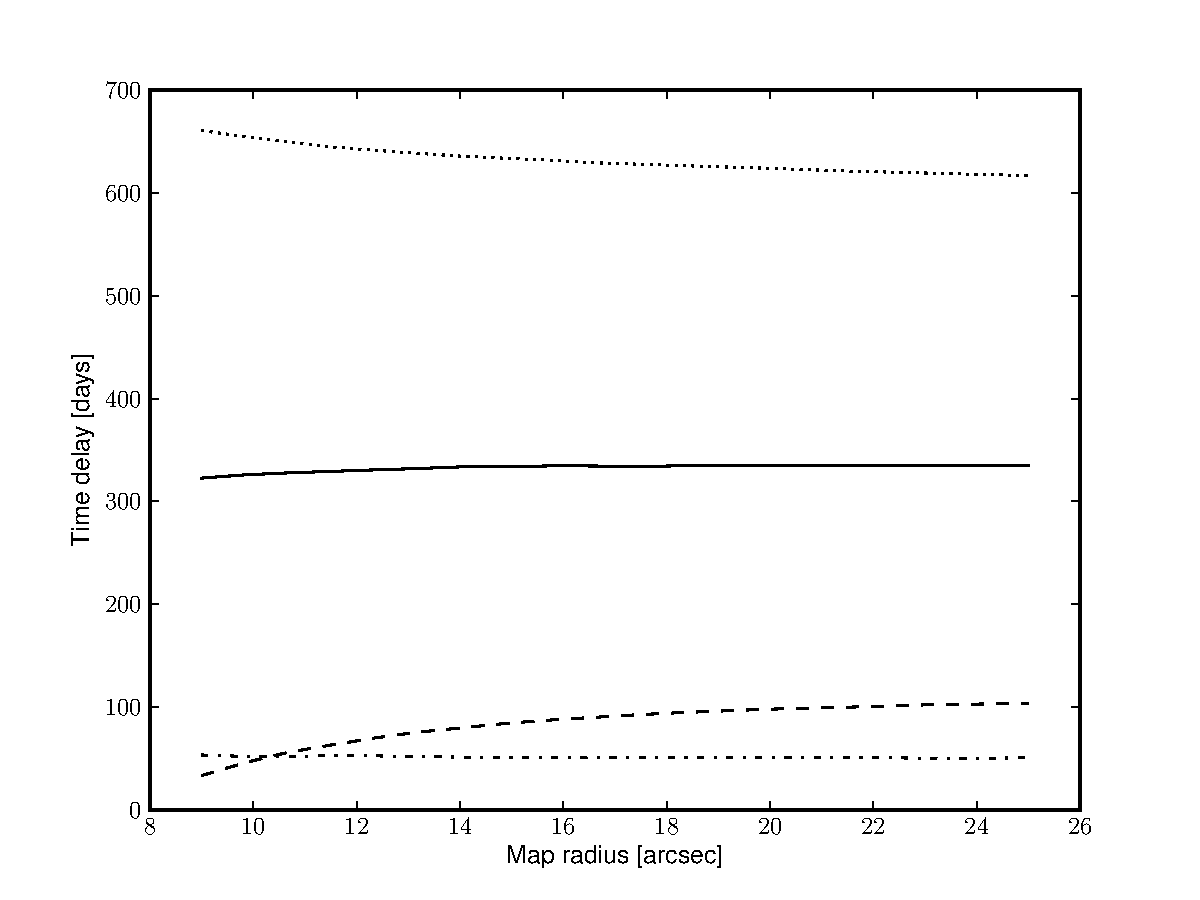
\includegraphics[width=.4\columnwidth]{tdconv_pr45.pdf}\hfil
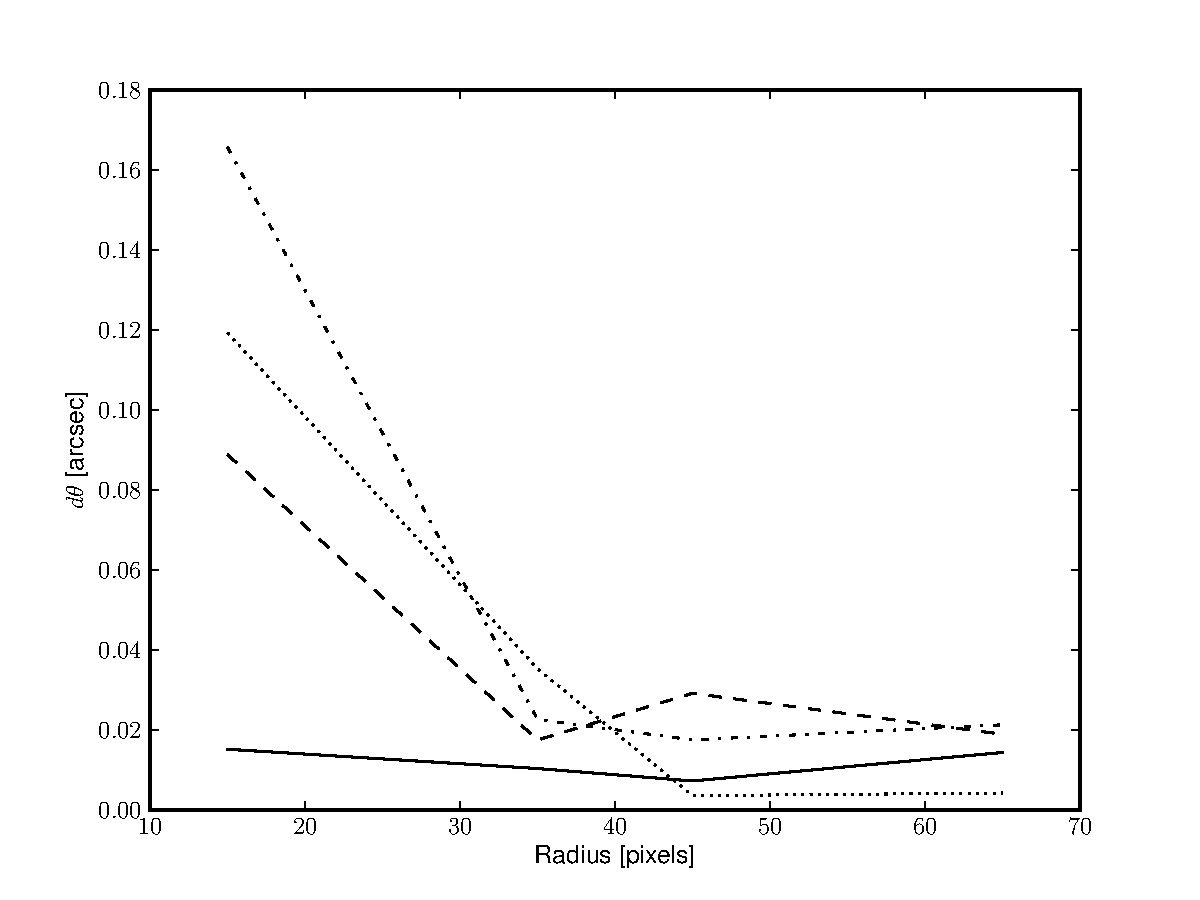
\includegraphics[width=.4\columnwidth]{imgpos_conv_mr20.pdf}
\end{center}
\caption{(left) Test for predicted time delay convergence as $\Rmap$
  changes.  $\Rpix=45$. After about $\Rmap=20$ most of the asymmetric
  mass is in the map.  (right) Test for predicted image position
  $\theta$ convergence as $\Rpix$ changes. $\Rmap=20$ arcsec.}
\label{raytracing convergence tests}
\end{figure}

\section{Mass reconstruction}

Reconstruct lenses \figref{reconstruction}.

\begin{figure}
\begin{center}
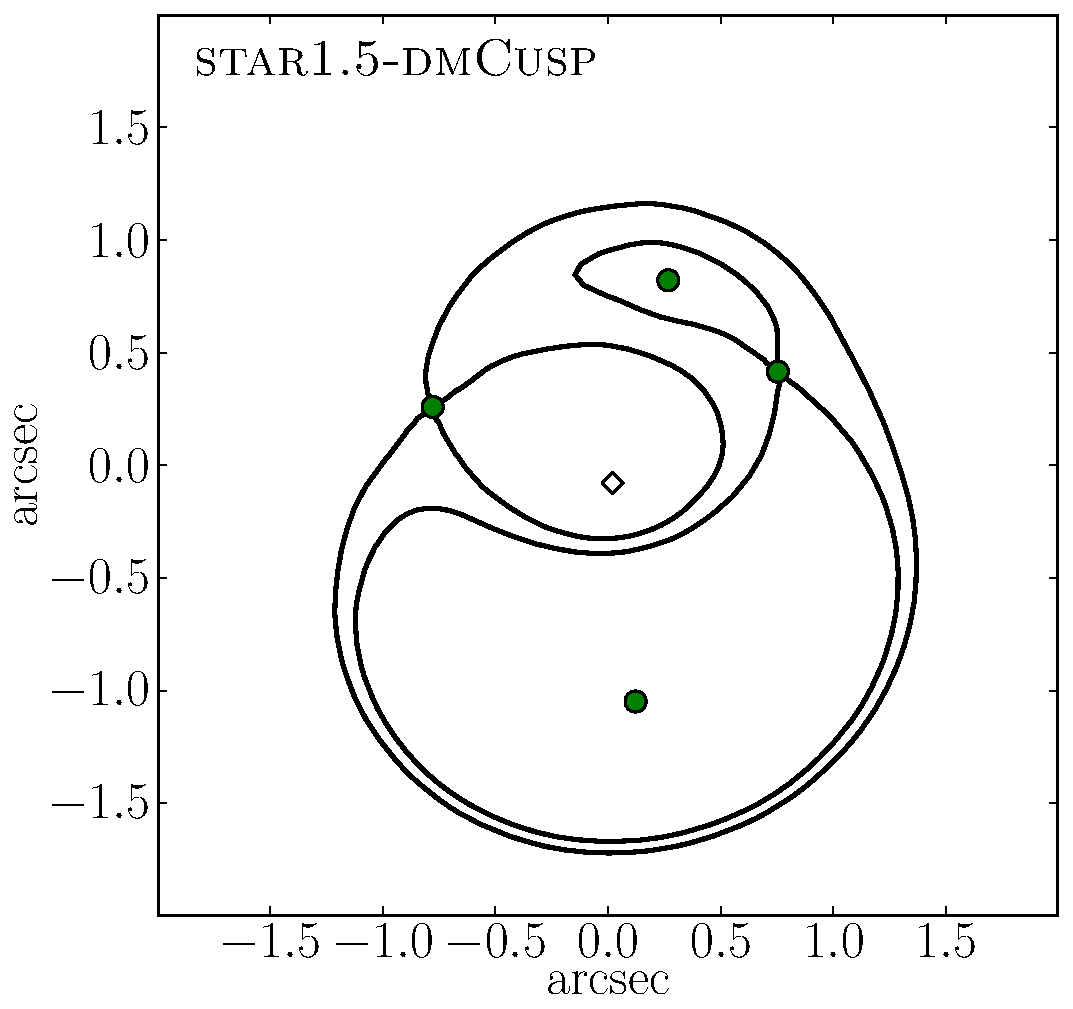
\includegraphics[width=.3\columnwidth]{BCQuadR1a_TmS-a.pdf}\hfil
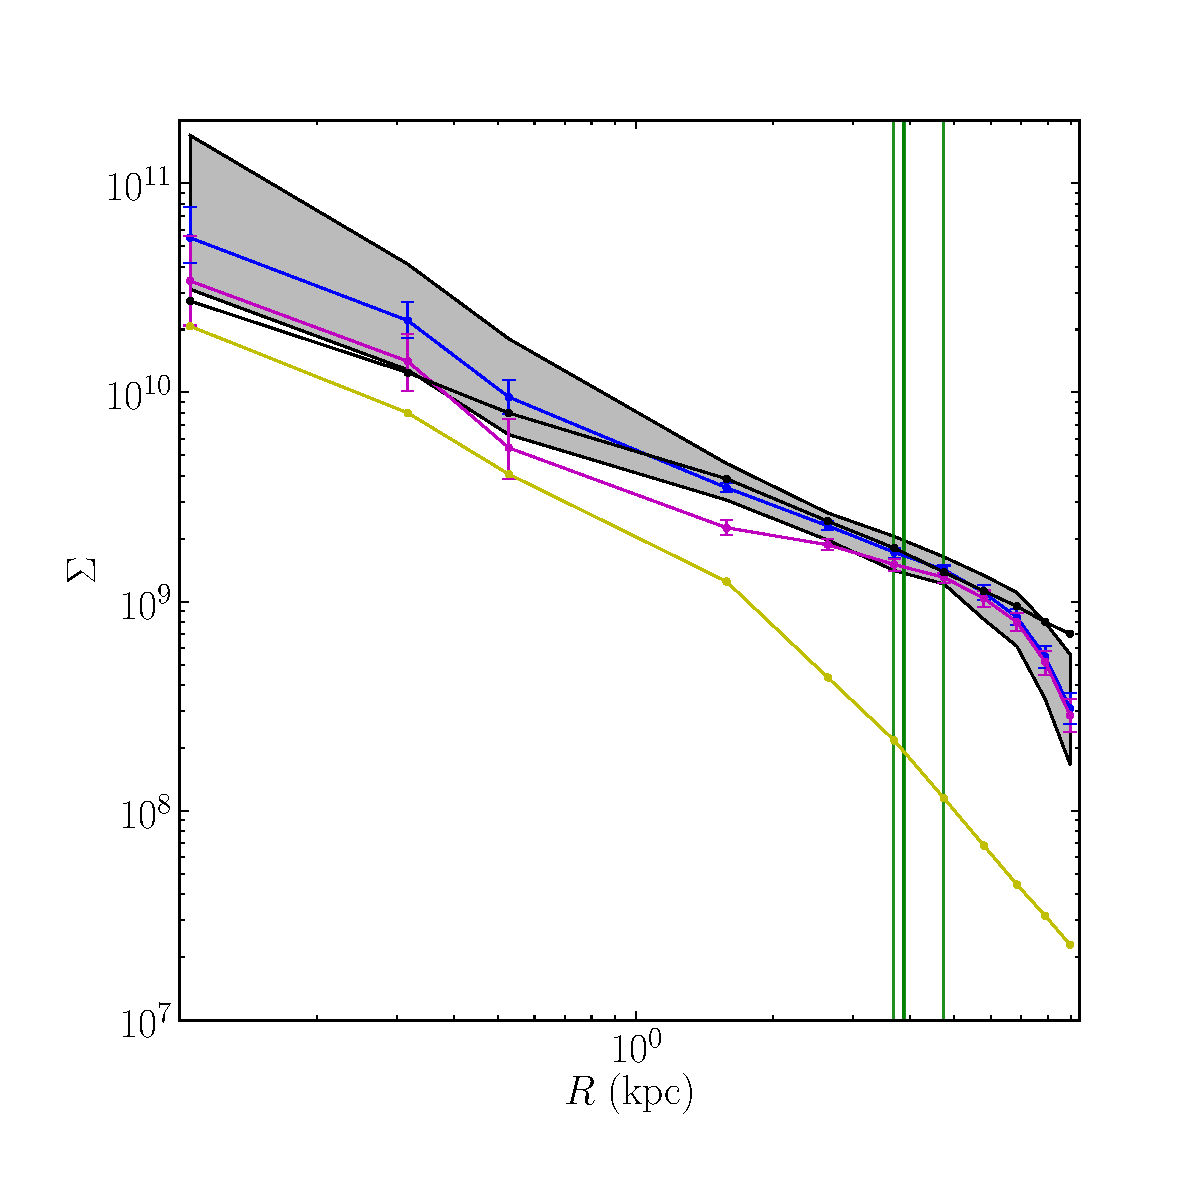
\includegraphics[width=.3\columnwidth]{BCQuadR1a_TmS-b.pdf}\hfil
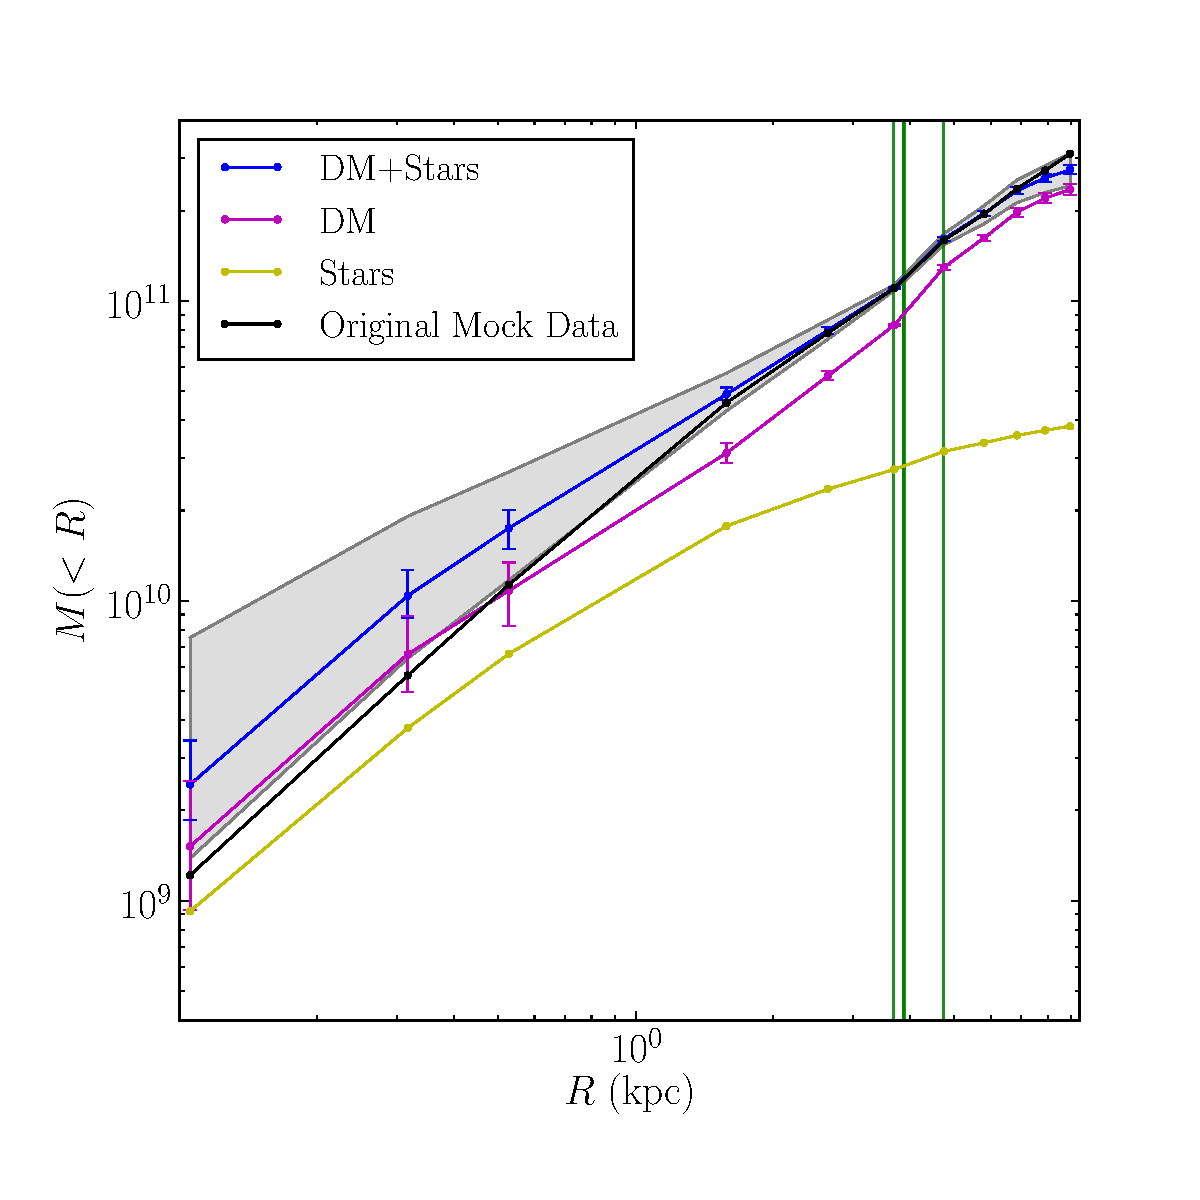
\includegraphics[width=.3\columnwidth]{BCQuadR1a_TmS-c.pdf}
\end{center}
\caption{A typical reconstructed lens.}
% Here we present a single quad
%   lens from the BC mock galaxy.  \textbf{(Left)} The arrival time
%   surface.  \textbf{(Middle)} The surface density. The magenta curve
%   represents the dark matter component, the yellow curve the stellar
%   component, and the blue curve is the sum of the two.  The black
%   curve comes from the original mass model used to create the lens.
%   The green vertical lines mark the radial positions of the
%   images. The higher resolution feature of \Glass\ has been used on
%   the central pixel allowing the steep profile to be captured.
%   \textbf{(Right)} The cumulative mass.}
\label{reconstruction}
\end{figure}

Quantify errors
\begin{equation}
\chi = \left(\frac
       {\Big\langle \int \left|\Delta\Sigma(\vec{\theta})\right|^2 \,
        d^2 \vec{\theta} \Big\rangle}
       {\int \Sigma^2(\vec{\theta}) \; d^2 \vec{\theta}}
       \right)^{1/2}
\end{equation}
and draw them, \figref{main results}.


\begin{figure}
\begin{center}
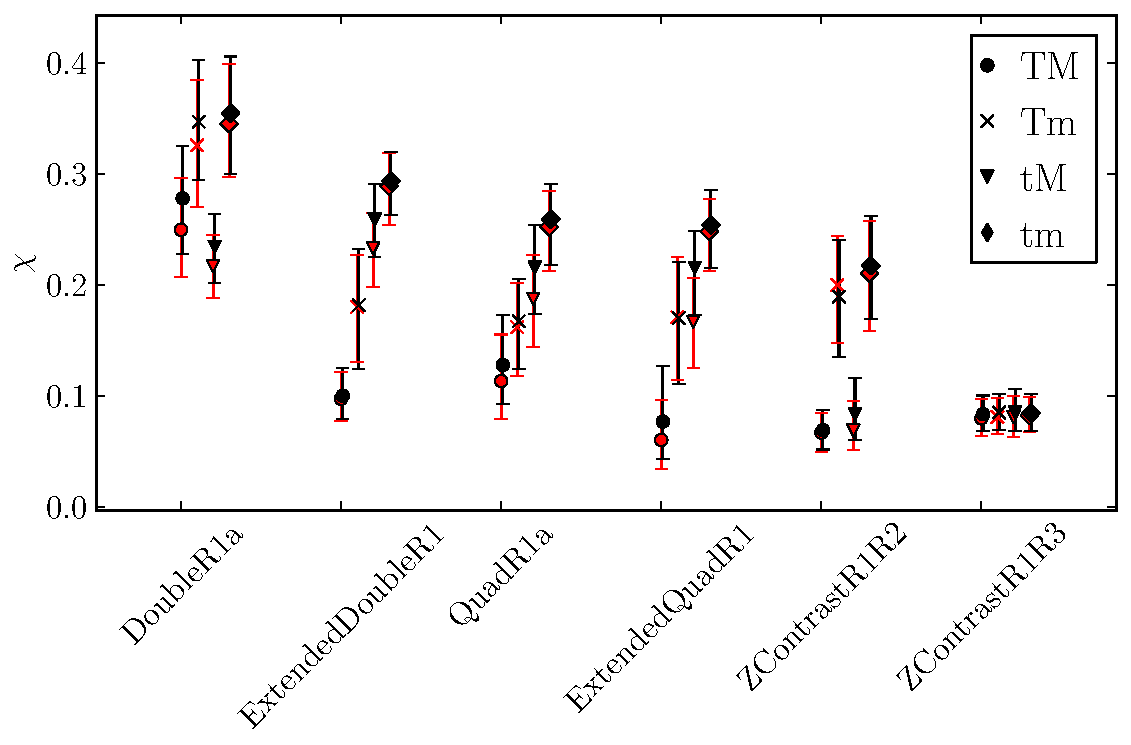
\includegraphics[width=.4\columnwidth]{AAchi2_profile.pdf}\hfil
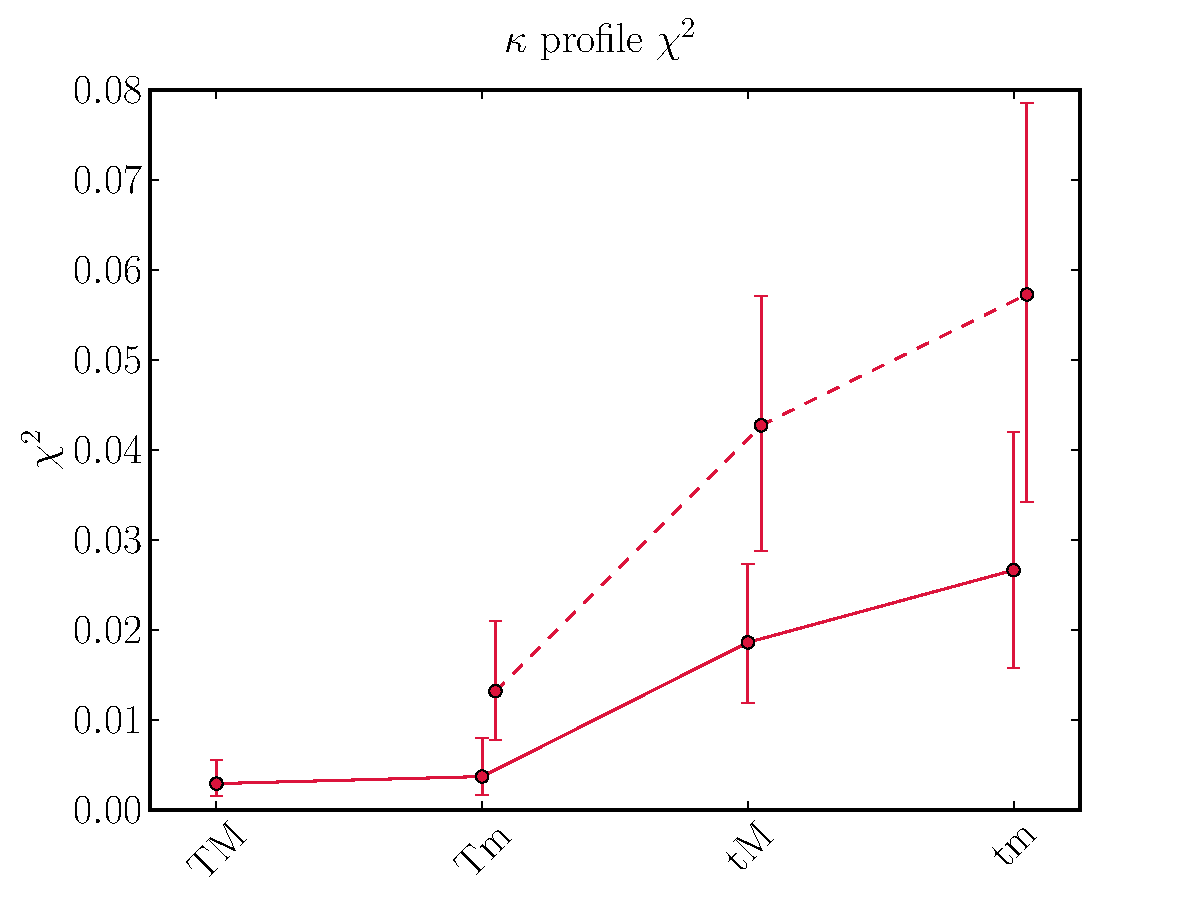
\includegraphics[width=.4\columnwidth]{BBchi2_profile.pdf}
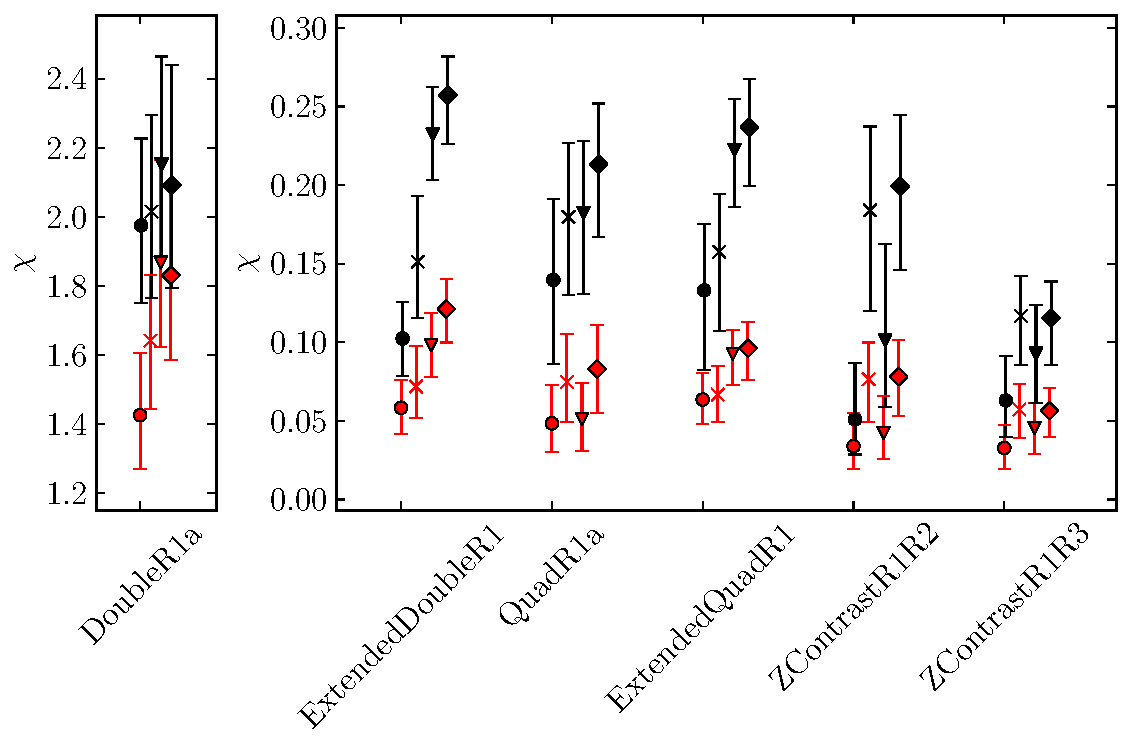
\includegraphics[width=.4\columnwidth]{ACchi2_profile.pdf}\hfil
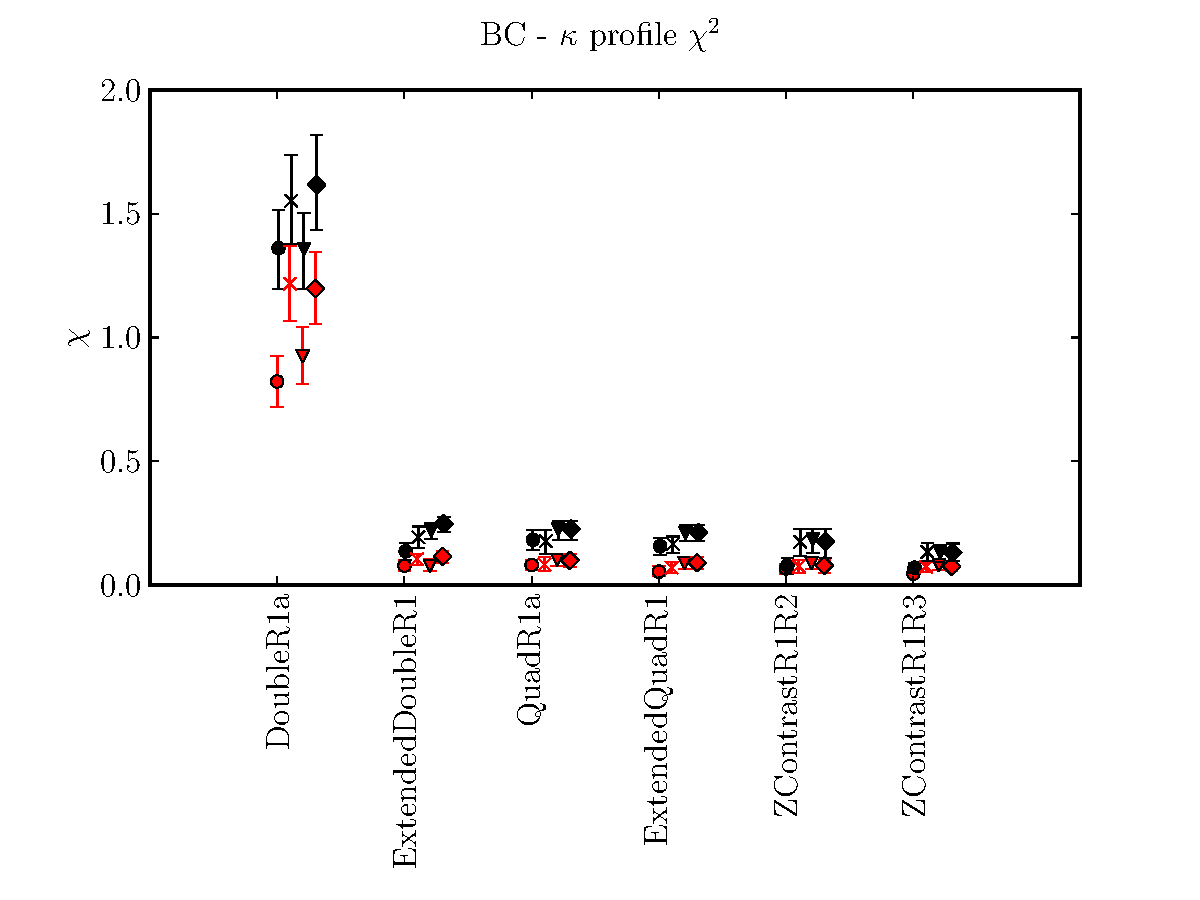
\includegraphics[width=.4\columnwidth]{BCchi2_profile.pdf}
\end{center}
\caption{The main results showing the quality of model recovery. Each
  panel corresponds to the named mock galaxy, whose parameters are
  listed in \tabref{mock galaxy params}. Within each panel are six
  groups of results for each of six lens morphologies. Each morphology
  considered the presence of time delays and a central image. The
  black markers are for tests that did not include the stellar mass as
  a lower bound constraint, while the red markers indicate where the
  stellar mass has been given.}
\label{main results}
\end{figure}

\section{Kinematics}

Velocity dispersion for different anisotropies, \figref{sigma-beta}.

\begin{figure}
\begin{center}
\includegraphics[width=.7\columnwidth]{BCQuadR1a_TmS-sb.pdf}
\end{center}
\caption{Estimated velocity dispersion as a function of the aperture
  size. The single quad lens model for the BC mock galaxy was
  deprojected and the mass profile fit assuming a Hernquist profile
  for the light. The top curve (blue) assumes a velocity anisotropy
  $\beta=1$, while the lower curve (green) assumes $\beta=0$. Given an
  independent estimate of the velocity dispersion, lensing can be used
  to place constraints on the velocity anisotropy.}
\label{sigma-beta}
\end{figure}



\bibliographystyle{mn2e}
\def\aap{A\&A}
\def\araa{ARA\&A}
\def\mnras{MNRAS}
\def\nat{Nature}
\def\nar{New Astr Rev}
\bibliography{ms}

\end{document}

